\documentclass[11pt,a4paper,oneside]{report}
\usepackage{graphicx}
\begin{document}
\begin{titlepage}


\title{CSP301 \\ Multiplayer Carrom}
\author{Rishabh Jain \\ 2010CS10241}
\date{}

\maketitle



\end{titlepage}

\setcounter{chapter}{1}

\section{Introduction}
The game of carrom is implemented in C++ using OpenGL for graphics and Stream Sockets for networking. We also made use of the C++ STL to exploit the functionality of vectors and queues. The code is as generic and as modular as possible. Different modules of the program such as physics, AI, networking or graphics were kept in different files. The program is extensively threaded to increase the performance and to keep the visuals smooth. For simultaneous networking between all the three clients and the server, parallelization was required. One thread is assigned to network with each of the three clients, so that even when one thread is blocked on receiving data, the other threads can carry out their respective jobs.

\section{Data Structure}

\begin{itemize}
\item{State Vector : This vector contains the positions and velocities of all the coins for a given instant.
}
\item{Event Queue : This queue contains all the critical events like hitting the striker and change of position of striker by the user.
}
\item{State Queue : This queue is a list of state vectors. It has the positions and the velocities of all the coins required to define the motion of the coins and striker at any time.}

\end{itemize}


\section{Threading}


\subsection{Common Threads}
\begin{itemize}

\item{Thread A : Event simulation \\}
This thread's job is to pop out an event from the Event Queue and use it to populate the State Queue. The State Queue would then be used by the graphics module to plot the states at the correct time. In case the Event Queue is empty, the thread is scheduled last and the thread waits for the queue to fill up. Also, when size of the State Queue exceeds an optimum value, the thread reschedules itself and waits for the size of the state queue to decrease. 
\item{Thread B : Graphics Thread \\}
This thread's job is to pop out a State Vector from the State Queue and plot it on the screen at the correct time. This thread also takes inputs from the mouse.

\end{itemize}
\subsection{Player Specific Threads}

\subsubsection{Server}

\begin{itemize}
\item{Thread C1 : Client Listener \\ }
This thread listens for messages from the Client number 1 (if it exists) and calls the function which was passed to it as a function pointer during the server initialization.
\item{Thread C2 : Client Listener \\ }
This thread listens for messages from the Client number 2 (if it exists) and calls the function which was passed to it as a function pointer during the server initialization.
\item{Thread C3 : Client Listener \\ }
This thread listens for messages from the Client number 3 (if it exists) and calls the function which was passed to it as a function pointer during the server initialization.
\item{Thread D : Port Hoster \\}
This thread runs in parallel for the clients to connect to it, while the main thread is sleeping for the specified timeout.
\item{Thread E : End of Event Listener\\}
This thread runs when the turn is passed to a client. So that if the response time of client is greater than some value it is disconnected from the server and the turn passed to the next player in the server.
\end{itemize}

\subsubsection{Client}
\begin{itemize}
\item{Thread C : This thread listens for messages from the Server and calls the function which was passed to it as a function pointer during its initialization.}
\end{itemize}

\section{Event Simulation}
In our model of event simulation, the future states are all pre-computed in parallel and stored in a State Queue. The graphics module then uses this queue to plot the states as and when required. The generating states and the displaying of states are independent. The advantage of this model is that the graphics runs without any delay. The graphics thread doesn't have to wait for the physics to be computed at each time instance.

\subsection{Problems Faced}
While populating the state queue its(state queue's) size can become too large to slow down the computer or even cause the program to run out of memory. Besides it can also make data accesses very slow. To avoid this problem the event simulation thread first checks the size of state queue if it exceeds a permissible value it relinquishes the CPU and gets scheduled to become the last thread in the run queue and starts another thread until the size of state queue reaches an optimal value.

\subsection{An example}
Taking an example of a game with two human players and 2 computer players, we will see the advantage of this model. First player 1 sitting in the server would make hsi move. The event, striker hit, would be sent to all the clients. Each client would populate the State Queue using this event that it has received from the server. The server would also announce that it is now player 2's chance. Computation and graphic display would take place at each client independently till all the coins stop. The server would then wait for player 2 to send data. After the coins have stopped for player 2, it would start taking user inputs. Player 2 can then position the striker and hit. Data would be sent to the server regarding this critical event. Since, there are only one client, the server does not have to send this data to any other client. Now, since the next and the next to next turns are computer turns, the server would two more critical events to the client, striker hit by player 3, and striker hit by player 4, which are generated by the AI. So, along with player 2's turn, even player 3 and 4's turns are sent to the clients. Computation would then proceed to calculate the states caused by all three events, and then diaplyed as and when required. After all these states have been displayed, it is now player 1's turn and this would then repeat. 

\section{Networking}
Our networking classes are very powerful in the sense that they give you full control over the stream socket by providing a clean and user-friendly interface.
\subsubsection{Server class}
Our Server class accepts following parameters as its constructor :
\begin{itemize}
\item{The port number to be listened}
\item{The function to be called when client binds to that port}
\item{The parameters to be passed to this function}
\item{The function to be called when the server receives a message with one of its parameters as the message recived}
\item{Addition data to be passed to this function}
\end{itemize}
For sending data you just nees to apply sendData method to an object of server class.
\subsubsection{Client class}
Our Client class accepts following parameters as its constructor :
\begin{itemize}
\item{The IP address to make a connection}
\item{The port number of that IP address}
\item{The function to be called when the client receives a message with one of its parameters as the message recived}
\item{Addition data to be passed to this function}
\end{itemize}
For sending data you just nees to apply sendData method to an object of client class.
\subsection{Implementation}
With the use of such easy to use classes we made possible any permution and combination possible for the state of players.
In our game player one has to be a computer or a human player and player 2,3,4 can be local computer players or human players or online computer players.
\subsection{Connection}
In our implementation client is required to give just the IP address of the machine on which it wants to connect. This is acheived by hosting the port between a specified range so that client knows on which ports to search for a server. So the client iterates over the range until it finds a connection. Often the client can connect to a port altough no game is running on it. To prevent this we send a pre-defined message from client to server and wait for a second for the server to respond. If the server responds within this time it means that the connection was valid. The server response is a pre-defined message concatenated with the information about the coins. As a result the initial positions and velocities of all the coins for all the players is the same.
\subsection{Working}
\subsubsection{Server to Client}
So when an event occurs on say a server, the server pushes the event into its Event Queue and broadcast the event in the form of a string message to all the clients connected to it if at all present and then finds out the next players whose turn it is. If that player is a client the server sends a message to tell the client that its his turn.
On the client side when it receives the event string, it forms an event out of it and pushes it into the Event Queue which is being looked upon by a thread. So while the Thread A and B are doing their job Thread C receives the message and comes to know that its his turn. But since the coins have started moving and there is an event in the queue and the state queue is not yet empty the mouse input remains blocked for the client. It is only after that all the coins have stopped that the input from the mouse would be taken.
\subsubsection{Client to Server}
Now that client has its mouse working it can generate an event. When an event is generated by it, the event gets pushed in the Event Queue and the event message is sent to the server in the form of a string. When the message is received by server it pushes this event into its queue and send it to the rest of the client to do the same.
\subsection{Error Handling}
During the client's turn we create a thread 'E' in server which listens for the end of event generation from the client for some timeout period. After that timeout period the thread forwards the chance to the next player and closes connection from the client, so that when the next time server tries to trigger an event in the client it fails and as a result pass the turn to the next player.
\section{Physics Implementation}
The job of the Thead A is to populate the State Queue but how ? It calls the functions defined in physics.cpp with the event as its parameters and it gets the position and velocities of the coins after a small time delta which it pushes into the state queue. It keeps on iterating over the positions and velocities until all the coins comes to rest.
\subsection{Working}
The physics part checks for every pair of coins if they are colliding and changes their velocities appropriately by conserving linear momentum and using the definition of coefficient of restitution. Next it checks the collision with the walls for all the coins. After doing all this check it updates the positions and the velocities using the frictin coefficient and applying Newtonian Mechanics.

\section{Sharing of Scores}
The scores are computed by the server and broadcasted to all the clients. This is done because the computation of scores and their sharing is a one time thing. In the sense that they are to be shared only when an event occurs. Therefore this policy of score sharing is good as it also avoids any error in scores as the scores correct themselves the next time server sends the scores to all the clients.

\section{Deciding the turn}
There should be a mechanism by which we are able to find the next player so that an event could only be generated by him.
To solve this problem we maintain an array of size four which contains the state of all the respective players. So the server/single player iterates over it, when it comes to know that an event has been generated. In case the current player is a local machine or a local computer, end of event is marked by storing a special strcture in the event queue. In case the current player is a client, it send a message to the server marking the end of its event generation.
If the server finds out that the next turn is of local machine or computer it just turns on its myTurn variable. In case the next turn is of a client the server sends a message triggermyTurnEvent or triggerAIEvent depending on whether the client is a human or a computer.

\section{Artificial Intelligence}
I am going to implement AI using the concept of ghost balls. A ghost ball is a ball where if a striker or a coin reaches with sufficient velocity than the coin under consideration is sure to get pocketed because the change in momentum occurs only along the line of collision. This pocketing scheme can be made recursive in the sense that the ghost ball become a new destination or say our new hole and we find a new ghost ball for it until we can find a ghost ball where our striker can reach.
Next problem I faced is where to place the striker on the line for a given ghost ball for that purpose one methosd is that we draw an arc from that ghost ball and mark the segments on the line where the shadow of the coins in between the ghost ball and the line lies. We cannot place our striker on these segments but anywhere else on this line. But this approach is cumbersome, instead we can increament the position of the striker by small amounts keeping it over the line. The advantage of this method is that its very easy to implement and its very rare that this method will fail.
\subsection{Level : Newbie}
When the level is newbie computer computes the biggest (a,b) pair where a denotes the index of the coin to be hit by the striker directly and b denotes the index of the pocket.
It finds out the ghost ball for this pair and provides sufficient velocity to the striker to reach the position of the ghost ball.
\subsection{Level : Amature}
In this level computer computes all the possible ghost balls then it selects that ghost ball where the angle between the line of collision and the velocity of the striker is minimum. As in this case maximum momentum would be transffered to the coin and also the effect of computational limitations like the precision of decimal numbers would become minimal.
\subsection{Level : Expert}
In this level computer finds out the 4 ghost balls each coressponding to a board wall for all (a,b) pairs discussed in newbiew level. It also calculates the strike angle for each ghost ball. Then it finds out the ghost ball Aghost with minimum strike angle and compares it to the strike angle of the ghost ball found in amature level. If the strike angle of ghost ball in amature level comes out to be minimum then this is our ghost ball, otherwise Aghost is the required ghost ball.
\subsubsection{Problems Faced}
Since the position determined for the ghost ball is a unique number and it is not necessary that in the process of simulation that position is acheived. This problem was solved by decreasing the time after which the next positions were calculated. But this in turn created another problem as now the display got slower as the number of states defined for the system increased. We overcame this problem by dropping some frames. So now all the coordinates are being calculated for close to perfect position of ghost ball as well as the balls in the display are moving at an acceptable speed.
\section{Rules of Carrom}
The red 'queen,' can be pocketed at any time after sinking your first piece but must be sunk before your last one. After pocketing the queen, you must sink one of your carrommen, thereby 'covering' it, into any pocket in the next shot, or she is returned to the center spot.

Once the queen is covered, whoever clears all their carrom men first wins the 'board'.

The winner of a board collects one point for each of the opponent's carrom men left at the finish and three points for the queen if covered by the winner (if covered by the loser, no-one gets those points). No more points are collected for the queen after your score reaches 22.

A game consists of 25 points or eight boards, whichever comes first.
\begin{itemize}
    \item{Sinking the striker costs you one piece and your turn. But, if you sink a piece in the same shot, then two come up and you shoot again.}

    \item{After sinking the striker, your opponent places the due piece(s) within the center circle. If you haven't sunk one yet, you owe one.}

    \item{If while shooting for the quee,n you also sink one of your carrom men in the same shot, the queen is automatically covered, no matter which went first.}

    \item{If the center spot is partially covered when replacing the queen or a jumped piece, the piece should cover as much red as possible. If totally covered, the piece is placed opposite the next player behind the red spot.}

    \item{If you sink your opponent's piece, you lose your turn. If you sink their last piece, you lose the board and three points.}

    \item{If you sink your last piece before the queen, you lose the board, three points and one point for each of your opponent's pieces left.}

\end{itemize}
\section{Input}
User can give inputs to the game either through the UI or from the terminal.
There can be four type of players none, human, local computer and client computer.
\begin{itemize}
\item{None :\\None is same as no player sitting on that position}
\item{Human :\\Human player expects human player to give inputs fromt the mouse}
\item{Local Computer :\\If the player is local computer all the computations are done on the server for that computer}
\item{Client Computer :\\If the player is client computer than the computaions for that player are done on the client machine}
\end{itemize}
\subsection{User Interface}
The user has to hit enter on the carrom executable file only.
\subsection{Terminal Input}
User has to type in 'n' for none, 'p' for person, 'c' for local computer followed by the level-1,2,3, i.e. c1,c2 or c3, default is c1, 'o' for client computer. All of these can be followed by the player name appended with a '-'. For example a standard valid entry would look like : ./carrom p-"Rishabh Jain" n c2-AI n.
If the user wishes to play  multiplayer he/she just needs to specify that player as a person or client computer and a port will begin listening for connections. For the second player to connect from the terminal the command should be of the form ./carrom j(level)-Name, where level is valid only when the client is a computer.

\newpage
\section{Screenshots}
\begin{figure}[htp]
\centering
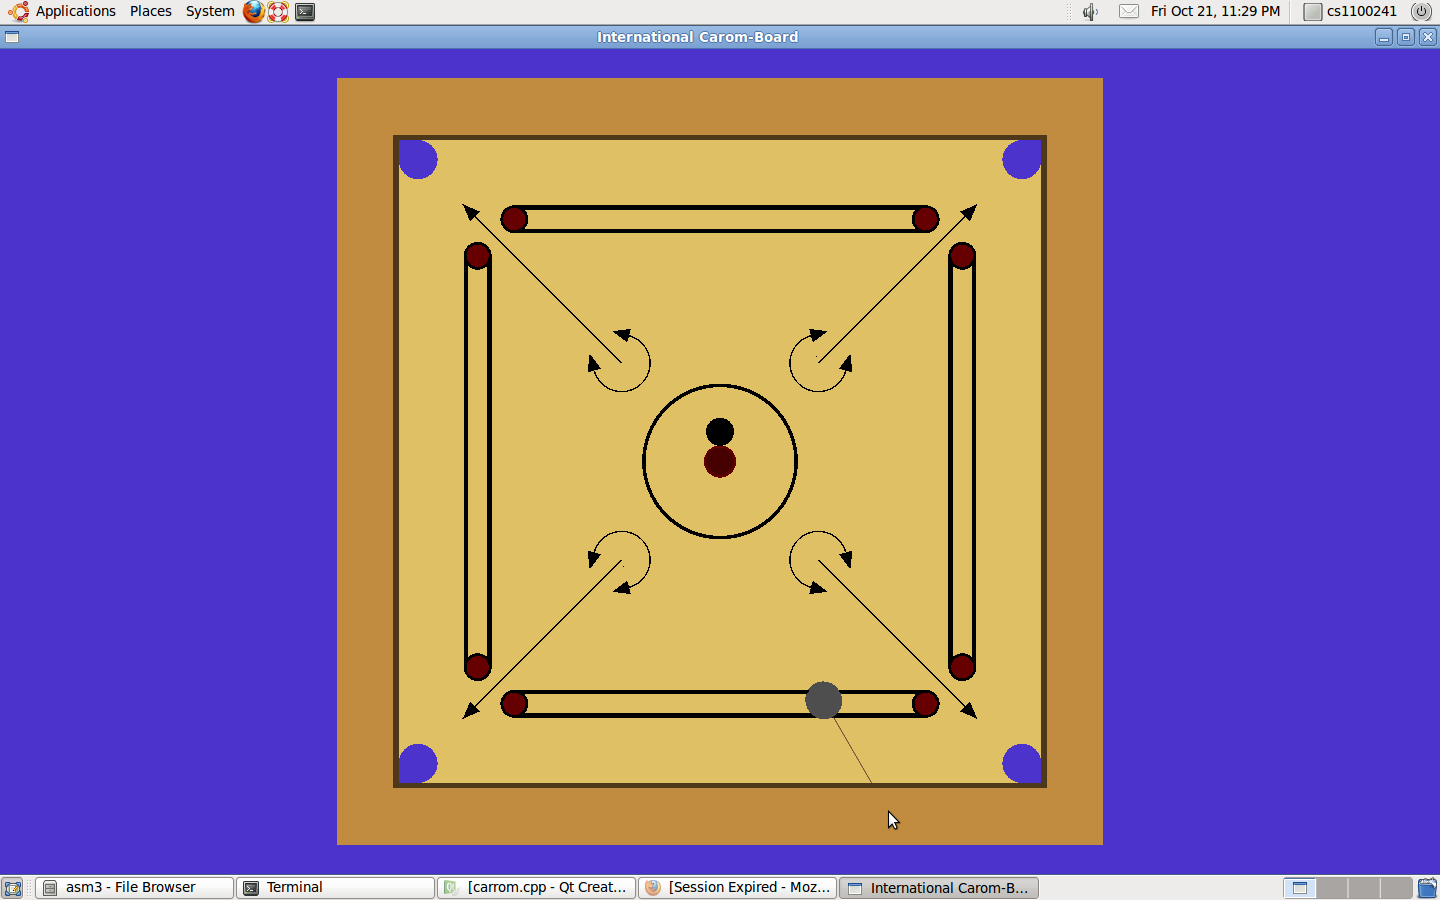
\includegraphics[scale=0.20]{Screenshot}
\caption{Screenshot-1}
\label{fig:Still from game}
\end{figure}

\begin{figure}[htp]
\centering
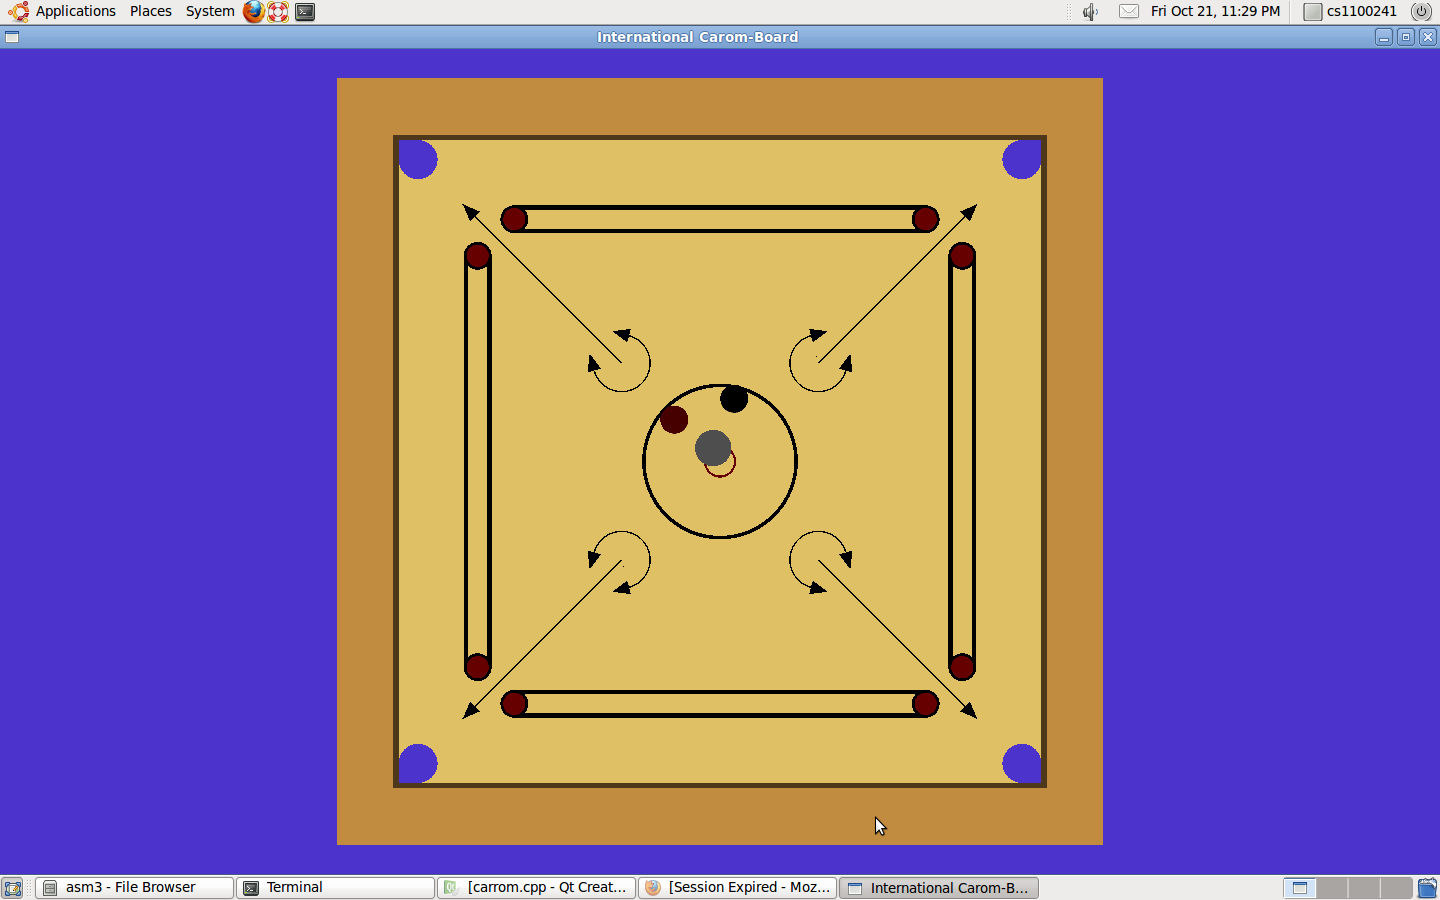
\includegraphics[scale=0.20]{Screenshot-1}
\caption{Screenshot-2}
\label{fig:Still from game}
\end{figure}

\begin{figure}[htp]
\centering
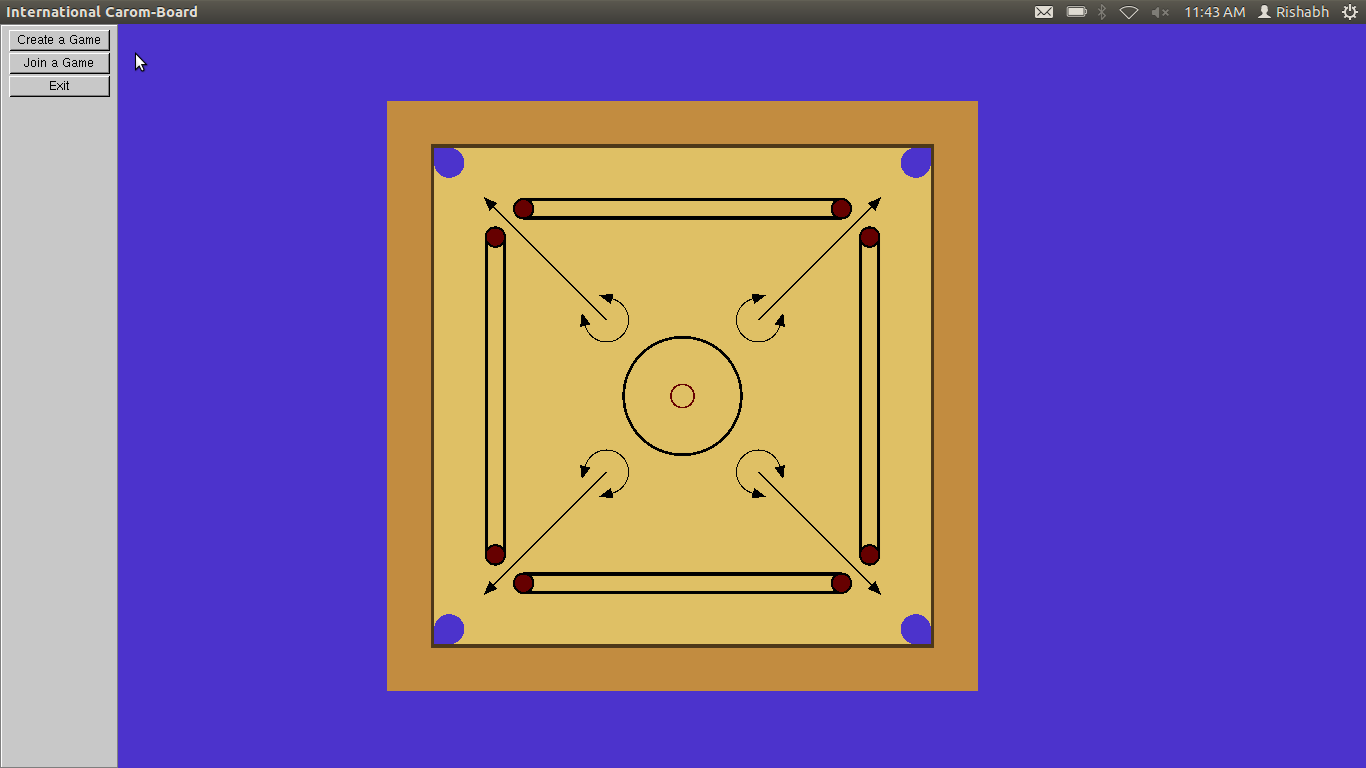
\includegraphics[scale=0.20]{Screenshot9}
\caption{Main Window}
\label{fig:Still from game}
\end{figure}

\begin{figure}[htp]
\centering
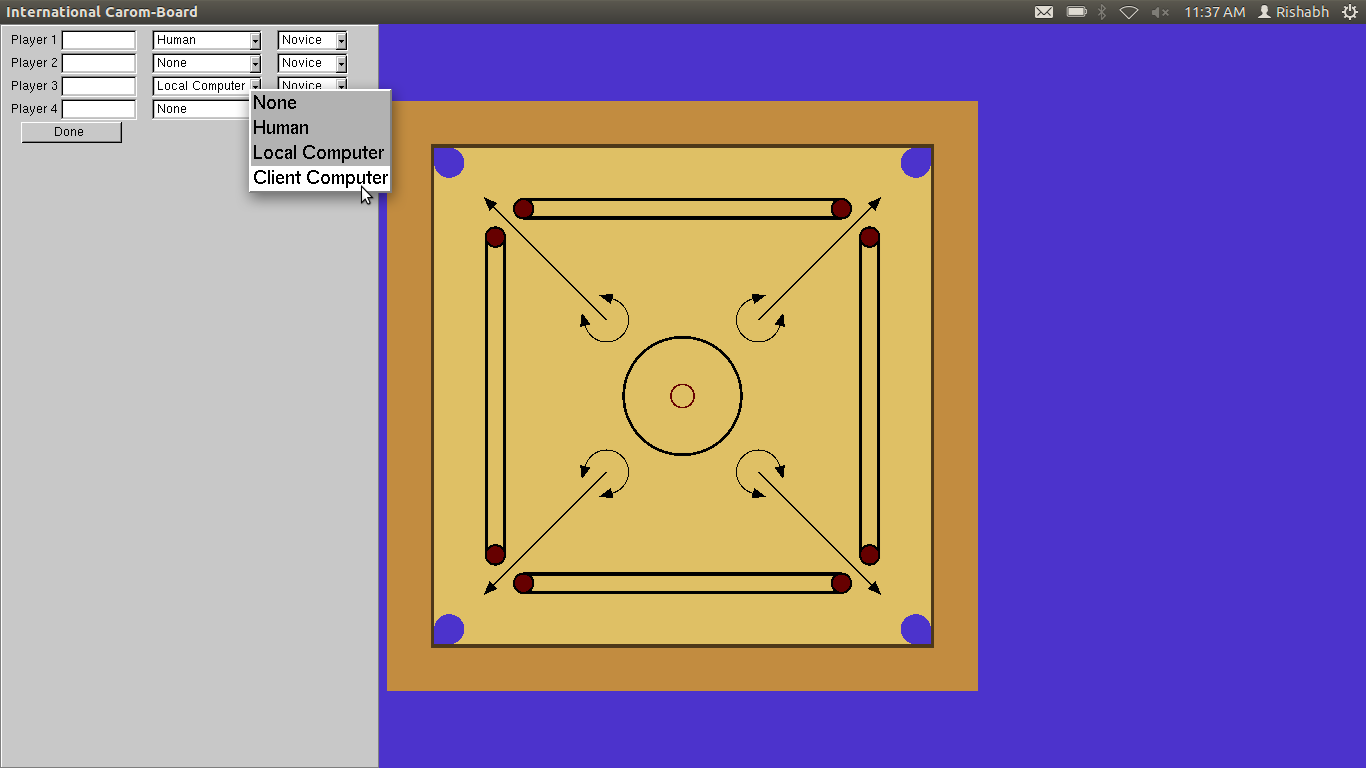
\includegraphics[scale=0.20]{Screenshot8}
\caption{Game Creation Window}
\label{fig:Still from game}
\end{figure}

\end{document}